\chapter{Lec 13 - Model Selection}

\section{Underfitting/Overfitting and learning parameters}
Suppose to have some data that we want to fit a curve to (regression problem). Let fit a polynomial of the form:
\[y = w_{0} + w_{1}x + w_{2}x^{2} + ... + w_{p}x^{p}\]
How can we choose the \textit{best} degree $p$?
\begin{center}
    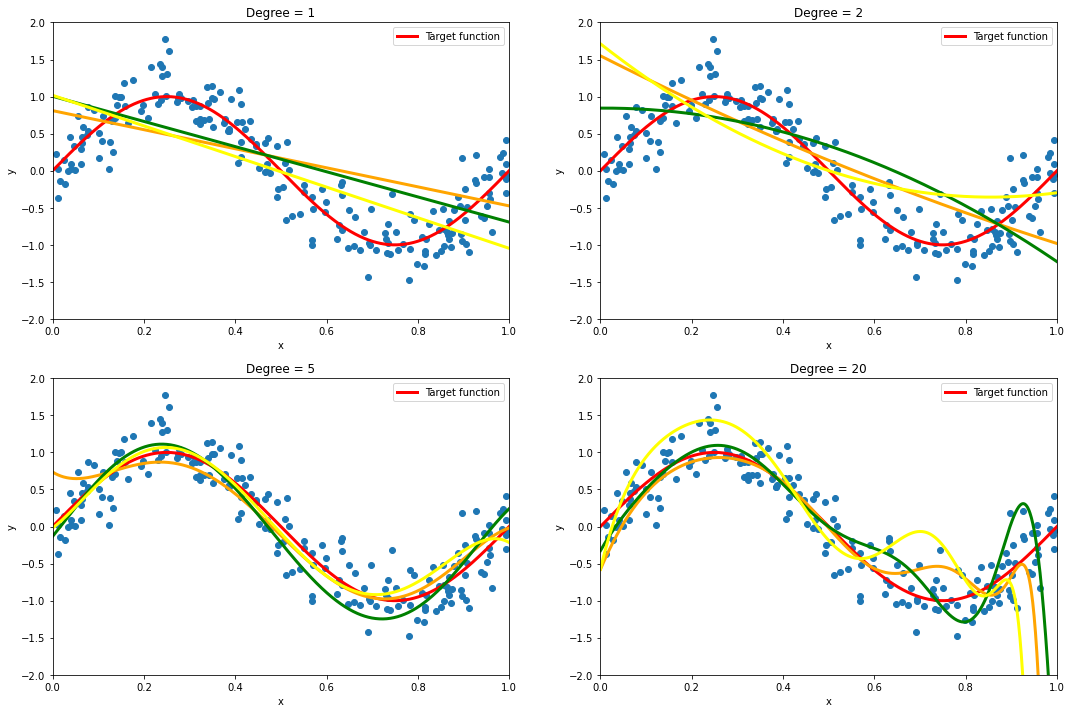
\includegraphics[scale = 0.35]{images/Model sel.png}
\end{center}
We can see that, by fitting different polynomial predictors (for different values of $p$), the complexity of the curve increases as the polynomial degree increases. For what concerning the training data, the \textbf{training} error decreases as $p$ increases, but when $p$ is too high the resulting curves cannot generalize well (\textbf{overfitting}). On the other hand, too low values of the polynomial degree can make the predictor to miss relevant relations between features (\textbf{underfitting}).\newline\newline
In order to understand more formally the concepts of overfitting and underfitting we can resort to the notions of \textbf{Bias} and \textbf{Variance}.
\begin{itemize}
    \item The Bias measures the \textit{distortion} of an estimate
    \item The Variance measures the \textit{dispersion} of an estimate
\end{itemize}
\begin{center}
    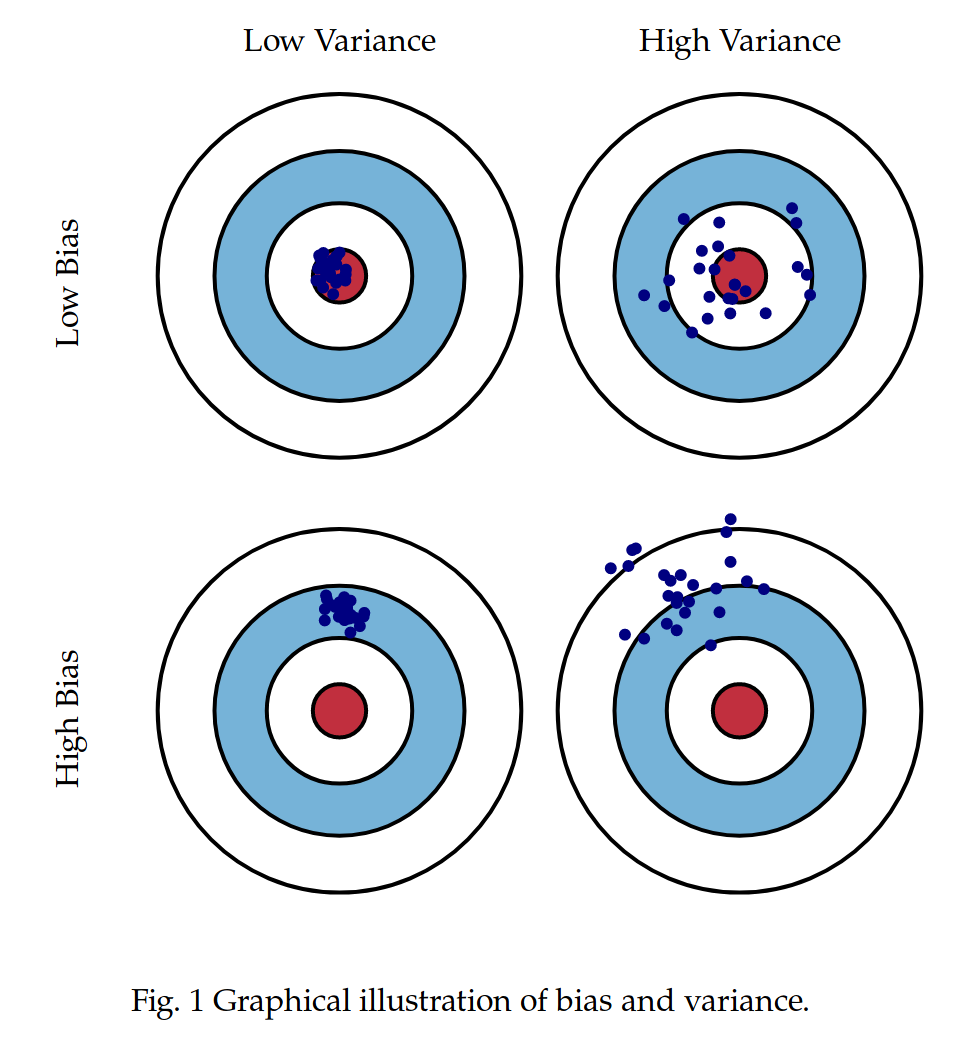
\includegraphics[scale = 0.2]{images/Bias-Variance.png}
\end{center}

\section{Bias-Variance Decomposition for Regression}
We can decompose the squared error of a given model in 3 terms:
\begin{itemize}
    \item Bias error term
    \item Variance error term
    \item irreducible error term
\end{itemize}
Let $y = f(\textbf{x}) + \epsilon$ be the target function, where $\epsilon$ is the error term \textit{selected} from a Gaussian distribution with zero mean and variance $\sigma^{2}$. We want to find a function $\hat{f}(\textbf{x})$ that approximates the target function $f(\textbf{x})$ as well as possible.\newline\newline
Given any pair $(\textbf{x}, y)$, the following holds:
\[E[(y-\hat{f}(\textbf{x}))^{2}] = (Bias[\hat{f}(\textbf{x})])^{2} + Var[\hat{f}(\textbf{x})] + \sigma^{2}\]
The formula says that the expected value of the squared error between the real output and the predicted output is equal to the sum of 3 terms:
\begin{itemize}
    \item The bias of the predictor $\hat{f}$ squared: $Bias[\hat{f}(\textbf{x})] = E[\hat{f}(\textbf{x})] - f(\textbf{x})$. It is the difference between the \textbf{expected} value of the predictor on $\textbf{x}$ and the true output $f(\textbf{x})$.
    
    \item The variance of the predictor $\hat{f}$: $Var[\hat{f}(\textbf{x})] = E[\hat{f}(\textbf{x}) - E[\hat{f}(\textbf{x})]]^{2}$.
    
    \item The irreducible error (variance of the noise $\epsilon$)
\end{itemize}
To obtain $E[\hat{f}(\textbf{x})]$ (the expected value of $\hat{f}$), for each $\textbf{x}$, we can train $n$ predictors $\hat{f}$ (over different small training examples) and compute the average of the predictions made by each model.\newline\newline
Note that the bias term will be higher if the expected value of the predictor is very different from the real output given by the target function. Furthermore, the variance error will be higher if the outputs of the different models used to compute $E[\hat{f}(\textbf{x})]$ are different from each other.\newline\newline
The learning goal is to find the best trade-off between bias and variance:
\begin{itemize}
    \item The bias error is produced by weak assumptions in the learning algorithm. For example, for very low $p$ the model is too simple and cannot capture the full complexity of the data (underfitting).

    \item The variance error is produced by an over-sensitivity to small      fluctuations in the training set. High variance can cause an algorithm to model the random noise in the training data, rather than the intended outputs (overfitting).
\end{itemize}
This estimation can be done only if we fix the target function, but in real applications this is not the case, because it is unknown. So, Bias-variance decomposition is a mathematical method for understanding and analyzing the errors made by a machine learning model, but it cannot be used to set the right value of the hyper-parameters. 

\section{Model selection and Hold-out}
Let's see some common ways to find the optimal hyper-parameters values using only the training data without resorting to any statistical formula.\newline\newline
The first method is the \textbf{Hold-out procedure}: The idea is to obtain a validation set (or hold-out set) $Va$ by splitting the training set $Tr$. Then, the fixed model is trained using examples in $Tr - Va$, trying different values of the hyper-parameters, and tested against the validation set. This procedure allows you to get an estimate of the error of the model on new unseen data.\newline\newline
In an operational setting, after the parameter optimization, the model is typically re-trained on the entire training set in order to boost effectiveness.

\subsection{K-fold Cross Validation}
An alternative approach for model selection (and evaluation) is the K-fold cross-validation:\newline\newline
\textbf{K-fold CV procedure:}\newline
\begin{enumerate}
    \item The training set is partitioned in $k$ disjoint sets $Va_{1}, ..., Va_{k}$ and $K$ different predictors $h_{1}, h_{2}, ..., h_{k}$ are trained by iteratively applying the Hold-out approach on the $k$-pairs ($Tr_{i} = Tr - Va_{i}, Va_{i}$).

    \item Final error is obtained by individually computing the errors of $h_{1},...,h_{k}$ on the corresponding validation set and averaging the results.
\end{enumerate}
The above procedure is repeated for different values of the hyper-parameters and the predictor with the smallest final error is selected.\newline\newline
The special case where $k = |Tr|$ (the validation sets are made of only one example) is called \textbf{leave-one-out} cross-validation.
\begin{itemize}
    \item For higher values of $k$, we have larger training sets, hence less bias, but smaller validation sets, hence more variance.

    \item For lower values of $k$, we have smaller training sets, hence more bias, but larger validation sets, hence less variance.
\end{itemize}

\section{Evaluation of unbalanced data - Beyond accuracy}
A common measure in machine learning to evaluate the performances of a model for what concerning the classification is the accuracy. Basically, it is the proportion of correct decisions. However, it is not appropriate when we have unbalanced data (e.g. the number of \textit{positive} examples is much lower than the number of \textit{negative} examples, or viceversa). This is because if we have a training set made of few positive examples (+) and a lot of negative examples (-) and we evaluate a model that always predicts (-), its accuracy will be very high even if it is a trivial predictor. So, we need to find other evaluation measures that take into account the unbalancing between data.\newline\newline
Before introducing these measures, let's define the contingency table:
\begin{center}
    \begin{tabular}{c|c|c}
         & Relevant & Not relevant  \\
         \hline
         Retrieved & True Positive (TP) & False Positive (FP) \\
         Not Retrieved & False Negative (FN) & True Negative (TN)
    \end{tabular}
\end{center}
The accuracy $\alpha$ is defined as follows:
\[\alpha = \frac{TP + TN}{TP + TN + FP + FN}\]

\subsection{Precision and Recall}
If relevance is assumed to be \textbf{binary-valued}, effectiveness is typically measured as a combination of:
\begin{itemize}
    \item \textbf{Precision}: 
    \[\pi = \frac{TP}{TP + FP}\]
    is the \textit{degree of soundness} of the system. It measures how many of the Retrieved classifications are actually Relevant.

    \item \textbf{Recall:}
    \[\rho = \frac{TP}{TP + FN}\]
    is the \textit{degree of completeness} of the system. It measures how many of the Relevant classifications are actually Retrieved.
\end{itemize}
In other words, Precision measures the proportion of positive predictions that are actually correct, while Recall measures the proportion of actual positive instances that were correctly predicted.\newline\newline
The choice between precision and recall often depends on the specific use case and the desired outcome of the model:
\begin{itemize}
    \item If the cost of false positive predictions is high, it may be desirable to prioritize precision. For example, in a medical diagnosis system, a false positive result could lead to unnecessary treatments, so a high Precision is desired.

    \item If the cost of false negatives is high, it may be desirable to prioritize recall. For example, in a fraud detection system, a false negative result could result in a missed fraud, so a high Recall is desired.
\end{itemize}

\subsection{F-Measure}
In some cases, it may be necessary to get a trade-off between Precision and Recall. This can be done using the \textbf{F-measure}, which is a weighted harmonic mean of the Precision ($\pi$) and Recall ($\rho$):
\[F_{\beta} = \frac{(1 + \beta^{2})\pi \rho}{\beta^{2}\pi + \rho}\]
If $\beta < 1$ it emphasizes Precision, while $\beta > 1$ emphasizes Recall. When $\beta = 1$, we obtain the so called F1 score:
\[F_{1} = 2\frac{\pi\rho}{\pi + \rho}\]

\section{Multi-class classification}
\textbf{Multi-class classification} consists of a classification task with more than two classes. It makes the assumption that each instance is assigned to only one label; for example, a fruit can either be an apple or an orange, but not both at the same time.\newline\newline
However, some models are defined only for binary problems (e.g. SVM), so how can the multi-class problem be reduced to a set of binary problems ?
\begin{itemize}
    \item The first strategy is the so called \textbf{one-vs-rest} strategy. It consists of fitting one classifier per class. For each binary classifier, its corresponding class is labelled as positive (+) and all the other classes as negative (-).\newline\newline
    The classification of new unseen examples is performed by classifying the example with all the classifier and selecting the one that matches with the highest response.\newline\newline
    One advantage of this approach is its interpretability. Since each class is represented  by only one classifier, it is possible to gain knowledge about the class by inspecting its corresponding classifier. This is the most common strategy and is a fair default choice.

    \item Another strategy is the \textbf{one-vs-one} strategy. It consists in fitting one classifier for each pair of classes. At prediction time, the class that received most votes is selected.\newline\newline
    Since it requires to fit $n\_classes * (n\_classes - 1 ) / 2$ classifiers, this method is usually slower than one-vs-rest. However, this technique may be advantageous for kernel algorithms which don't scale well with $n\_samples$. This is because each individual learning problem only involves a small subset of examples, while with one-vs-rest method the complete dataset is used $n\_classes$ times.
\end{itemize}

\section{Evaluation of Multi-class classification}
A very intuitive way to show the results of a multi-class predictor is using the \textbf{confusion matrix}.
\begin{flushleft}
    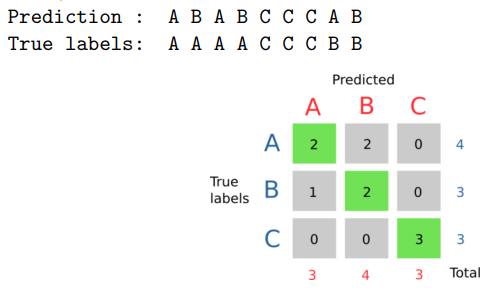
\includegraphics[]{images/Confusion matrix.png}
\end{flushleft}
It is a table with true labels over the rows and predicted labels over columns. Each cell over the diagonal contains the number of times the true label was correctly predicted.\newline\newline
Then, we can compute the Precision and Recall measures for the multi-class problem according to this matrix:
\begin{itemize}
    \item Precision can be calculated separately for each class. For each column, we take the number on the diagonal and we divide it by the sum of all the numbers in the column.
    \begin{itemize}
        \item $prec\_A: \,\, 2/3 = 0.67$
        \item $prec\_B: \,\, 2/4 = 0.50$
        \item $prec\_C: \,\, 3/3 = 1$
    \end{itemize}

    \item Recall can be computed separately for each class. It is the value on the diagonal divided by the sum of the values on the row.
    \begin{itemize}
        \item $recall\_A: \,\, 2/4 = 0.50$
        \item $recall\_B: \,\, 2/3 = 0.67$
        \item $recall\_C: \,\, 3/3 = 1$
    \end{itemize}
\end{itemize}
To extract a single number from the Precision, Recall or F1-score of the model, it is common to adopt two different kinds of average:
\begin{itemize}
    \item The first is to compute the score separately for each class and taking the average value (\textbf{macro averaging}).

    \item The second is to compute the measure from the grand total of the numerator and denominator (\textbf{micro averaging}). For our Recall example, the micro average is the following:
    \[\frac{2 + 2 + 3}{4 + 3 + 3 } = 0.636\]
\end{itemize}

